\documentclass[12pt]{aghdpl}
\usepackage[utf8]{inputenc}

\usepackage{enumerate}
\usepackage{listings}
\usepackage{pgfplots}
\usepackage{tikz}
\usepackage{svg}
\usepackage{graphicx}
\usepackage{setspace}
\usepackage{makecell}
\usepackage{caption}
\usepackage{subcaption}
\usepackage{pgf-umlsd}
\usepackage{epstopdf}
\usepackage{bytefield}
\usepackage{amsmath}
\usepackage{csquotes}
\usepackage[nottoc,numbib]{tocbibind}
\usepackage[section]{placeins}
\usepackage{tgtermes}
\usepackage{color}
\usepackage{hyperref}
\usepackage{sourcecodepro}

\usetikzlibrary{shapes.geometric}
\usetikzlibrary{arrows.meta}
\usetikzlibrary{decorations.text}
\usetikzlibrary{positioning}
\usetikzlibrary{fit,shapes}

\hypersetup{
colorlinks,
citecolor=black,
filecolor=black,
linkcolor=black,
urlcolor=black
}

\lstloadlanguages{TeX}
\lstset{
basicstyle=\footnotesize\ttfamily,
breaklines=true,
frame=single,
frameround=tttt}

\definecolor{lightred}{rgb}{1,0.7,0.71}

\begin{document}

    \thispagestyle{empty}
{\fontfamily{qtm}\selectfont
\begin{figure}[htbp]
    \centering
    \includegraphics[scale=1.5]{img/agh-logo.pdf}
\end{figure}

\centerline{\small\textbf{AKADEMIA GÓRNICZO-HUTNICZA IM. STANISŁAWA STASZICA W KRAKOWIE}}
\vspace{1em}
\centerline{\small\textbf{WYDZIAŁ INFORMATYKI, ELEKTRONIKI I TELEKOMUNIKACJI}}
\vspace{1em}
\centerline{\small INSTYTUT Informatyki}
\vspace{2em}
\centerline{\Large Praca dyplomowa}
\vspace{2em}
\centerline{\textit{\large Validation of QUIC protocol usefullness in interactive communication}}
\vspace{1em}
\centerline{\textit{\large Ocena przydatności protokołu QUIC w komunikacji interaktywnej}}
\vspace{3em}

\begin{table}[h]
    \begin{tabular}{l l}
        Autor             & Michał Śledź              \\
        Kierunek studiów: & Informatyka               \\
        Opiekun pracy:    & dr inż.\ Łukasz Czekierda \\
    \end{tabular}
\end{table}

\null
\vfill
\centerline{Kraków, 2021}
}
    \clearpage

    \tableofcontents
    \clearpage

    \section{Introduction}
\label{sec:introduction}

An interactive communication is bidirectional data exchange between people or people and machines.
It consists of two or more participants and has to be responsive meaning the result of performed action is delivered almost immediately.
In many cases interactive communication has to be also secure and reliable.
Examples of interactive communication are controlling remote robot in tele-surgery, doing exercises in tele-rehabilitation and
some types of multimedia sessions e.g.\ video conference, collaborative work or chat.
On the other hand to interactive communication does not belong exchanging emails (time between subsequent messages is too big) or
video on demand and streaming (they are not bidirectional).

Years of researches, protocol improvements and network devices optimizations have made interactive communication really fast.
We can talk with another person almost in the real time with a delay of several milliseconds.
Having said that it is perfectly correct to ask a question whether communication can be even faster, more effective and reliable and whether it is still worth to make improvements while we already have well prospering ecosystem.
In 2006 Prof.\ Edward Delp said:
\begin{displayquote}
    Is video coding dead?
    Some feel that, with the higher coding efficiency of the H.264/MPEG-4 Advanced Video Coding (AVC) standard (2x as compared to MPEG-2), perhaps there is not much more to do.
    I must admit that I have heard this \textquote{compression is dead} argument at least four times since I started working in image and video coding in 1976.\cite{4015574}
\end{displayquote}
Despite the fact that we are able to achieve very good performance in video conferencing systems there is still much to do.
Serious gaming, tele-surgery and tele-rehabilitation are all subject to tactile internet in which reliability, security and low latency are fundamental.
In such cases delay of 1 ms is desirable~\cite{the-tactile-internet}.

On the other hand, complexity of current standards makes them hard to implement, monitor and maintain.
One of them is WebRTC which uses over 10 different protocols and leaves implementation of signalling plane to the user.

QUIC is a new transport protocol standardized in RFC 9000 on May in 2021 and provides interesting and promising set of features.
%Its integration with TLS 1.3 significantly reduces connection establishment time while stream multiplexing in a single connection resolves head of line blocking problem of HTTP/2.
%QUIC introduces also special connection identifiers that prevents from additional handshakes in case of network switching and defines own flow control and congestion control mechanisms that are based on TCP ones.
%QUIC packets are encapsulated in UDP datagrams which makes QUIC user level protocol i.e.\ there is no need to modify kernel implementation to provide operating system with support for QUIC\@.
%
QUIC is mostly deployed in conjunction with a new version of HTTP called HTTP/3 and is intended to replace TCP and HTTP/2.
Therefore most publications are focused on web domain comparing QUIC and HTTP/3 with TCP/TLS and HTTP/2.

However, it turns out that a lot of QUIC features mainly stream multiplexing, pluggable congestion control, integration with TLS 1.3
or enhanced connection establishment mechanism can be useful in other domains.
As a result a number of IETF drafts emerged to expand QUIC to new areas.
The most important one is \textit{An Unreliable Datagram Extension to QUIC}.
It allows for combining reliable and unreliable data exchange in the same QUIC connection.

This document tries to answer a question whether QUIC can introduce significant improvement in terms of interactive communication.
To this end, analysis of QUIC encryption, loss detection and flow control mechanisms as well as number of tests and experiments have been performed.

The structure of this document is as follows.
Section~\ref{sec:state-of-the-art} presents state of the art and defines problems that will be addressed in this document.
Section~\ref{sec:quic-overview} introduces basic concepts of QUIC and compares QUIC to other transport protocols.
Section~\ref{sec:quic-in-webrtc} presents how QUIC can simplify WebRTC protocol stack.
It also describes packet encryption process in QUIC, answers the question if header encryption introduces significant overhead to the whole packet encryption and compares QUIC encryption process with RTP one.
Section~\ref{sec:datagrams} is dedicated to DATAGRAM frames in QUIC -- how they work and behave in different scenarios.
Section~\ref{sec:conclusions} concludes this document.

    \clearpage
    %! suppress = EscapeAmpersand


\chapter{QUIC overview}
\label{ch:quic-overview}
QUIC is a connection-oriented, multistream protocol that uses UDP/IP under the hood.
It is integrated with TLS and provides own congestion control and flow control mechanisms.
Data sent over QUIC is delivered in a reliable way.

This section outlines main features of QUIC and compares QUIC to the other transport protocols.


\section{Connection}
\label{sec:connection}
A QUIC connection is shared state between a client and a server.
It consists of connection parameters like initial flow control limit or initial maximal number of streams and
shared secret used for encryption.
Each connection possesses a set of connection identifiers each of which identifies the connection.
The role of connection IDs is to make QUIC connection resilient for changes in addressing at lower protocol layers (UDP, IP).
In such scenarios, as long as there is an alternative network path QUIC can migrate to it without restarting the connection.
As an example one could open UDP socket, establish QUIC connection, start sending packets using open socket and after some time
switch UDP socket to another one (e.g.\ because of moving train) without re-establishing QUIC connection or creating a new one.

Using a connection ID is optional and an endpoint can decide to use zero-length connection ID when a connection ID is not needed to route packets to the correct endpoint.
However, choosing zero-length connection ID makes it impossible to use some QUIC features like mentioned above
connection migration.


\section{Data structures}
\label{sec:quic-data-structures}
The most outer entity in QUIC is a packet.
QUIC defines different types of packets each of which consists of a header followed by a type-specific payload.

Header can take long or short form.
Packets with long headers are used at the beginning of the communication, before establishing 1-RTT keys.
After negotiating cryptographic context QUIC switches to the packet type with short header form for minimizing data sent
through the network.
Short Header consists of miscellaneous flags which take one byte, destination connection ID and packet number.
Total size of Short Header depends on using zero-length connection ID and is from 2 to 25 bytes allowing for saving
bandwidth in scenarios when some QUIC features like connection migration are not needed.
Short header form is illustrated in figure~\ref{fig:short-header-format}.

\begin{figure}[h]
    \centering
    \begin{bytefield}[bitwidth=4em]{8}
        \bitheader{0-7} \\
        \bitbox{1}{\tiny header form} & \bitbox{1}{\tiny fixed bit} & \bitbox{1}{\tiny spin bit} & \bitbox{2}{\tiny reserved bits} & \bitbox{1}{\tiny key phase} & \bitbox{2}{\tiny packet number length} \\
        \wordbox{1}{\tiny destination connection ID (0 - 160)} \\
        \wordbox{1}{\tiny packet number (8 - 32)}
    \end{bytefield}
    \caption{QUIC Short Header format}
    \label{fig:short-header-format}
\end{figure}

Long Header additionally includes version, destination connection ID length, source connection ID
length and source connection ID fields.
It does not include packet number field and its flags differ a little comparing to the Short Header but they also take 1 byte.
Total length of Long Header also depends on using zero-length connection ID and is from 7 to 47 bytes.
Long header form is illustrated in figure~\ref{fig:long-header-format}.

\begin{figure}[h]
    \centering
    \begin{bytefield}[bitwidth=4em]{8}
        \bitheader{0-7} \\
        \bitbox{1}{\tiny header form} & \bitbox{1}{\tiny fixed bit} & \bitbox{2}{\tiny long packet type} & \bitbox{4}{\tiny Type-Specific Bits} \\
        \wordbox{4}{\tiny Version (32)} \\
        \wordbox{1}{\tiny Destination Connection ID Length} \\
        \wordbox{1}{\tiny destination connection ID (0 - 160)} \\
        \wordbox{1}{\tiny Source Connection ID Length} \\
        \wordbox{1}{\tiny Source Connection ID (0 - 160)}
    \end{bytefield}
    \caption{QUIC Long Header format}
    \label{fig:long-header-format}
\end{figure}

QUIC defines following types of packets that use long header form: Version Negotiation, Initial, 0-RTT, Handshake, Retry and one packet type that uses short header form called 1-RTT\@.

Payload form depends on a packet type.
It includes type-specific fields which are in most cases followed by QUIC frames.
Payload can include many frames and many frame types.
Some of the QUIC frames are: PING, ACK, CRYPTO or STREAM\@.
Different frame types can appear only in specific packet types.
For example STREAM frame can only be included in 0-RTT or 1-RTT packets while CRYPTO frame can appear in Initial, Handshake or 1-RTT packets.
Version Negotiation and Retry packets does not include any QUIC frames at all.


\section{Encapsulation}
\label{sec:udp-based}
QUIC packets are directly encapsulated into UDP datagrams.
One UDP datagram can coalesce multiple QUIC packets provided that each of them possesses the same connection ID and contains length field.
If a packet does not contain length field it has to be placed at the end of UDP datagram which implies there can be only one such packet.
Packets that contain length field are Initial, 0-RTT and Handshake while packets without length field are Retry, Version Negotiation
and 1-RTT\@.
It is also important that there is no situation where Retry or Version Negotiation packet is coalesced with another packet.
One of the advantages of coalescing QUIC packet is reduction of number of UDP datagrams needed to establish QUIC connection.
Example encapsulation is shown in figure~\ref{fig:quic-encapsulation}.

\begin{figure}[h]
    \centering
    \begin{bytefield}[bitwidth=4em]{8}
        \begin{leftwordgroup}{\small UDP \\ \small header}
            \bitbox{4}{\small Source Port} & \bitbox{4}{\small Destination Port} \\
            \bitbox{4}{\small Length } & \bitbox{4}{\small Checksum}
        \end{leftwordgroup} \\
        \begin{leftwordgroup}{\small UDP \\ \small payload}
            \wordbox{1}{\small QUIC Long Header packet} \\
            \wordbox{1}{\small QUIC Long Header packet} \\
            \wordbox{1}{\small QUIC Short Header packet}
        \end{leftwordgroup}
    \end{bytefield}
    \caption{QUIC encapsulation into UDP datagram}
    \label{fig:quic-encapsulation}
\end{figure}

Encapsulating QUIC packets into UDP datagrams makes QUIC user-level protocol which means it can be implement as a usual
library without modifying operating system kernel.
Moreover, existing middleboxes see QUIC packets as usual UDP datagrams and do not require providing support for a new protocol.
On the other hand, a lot of government institutions as well as companies block incoming or outgoing UDP traffic and allow
only for communication via TCP or TLS on port 443.


\section{Security}
\label{sec:security}
QUIC is integrated with TLS 1.3 providing confidentiality, integrity and authenticity of its packets.
Confidentiality means that no one is able to decrypt data being sent to the other endpoint, integrity means that no one
is able to modify this data and authenticity means that each endpoint can verify identity of
its peer to be sure that it is communicating with proper entity.
Integration with TLS 1.3 is described in details in RFC 9001~\cite{rfc9001}.
Both transport and cryptographic parameters are negotiated in a single connection handshake which results in
reduction of connection establishment time (see~\ref{sec:connection-establishment}).
Unlike in TLS over TCP, QUIC does not carry TLS records.
Instead, TLS handshake and alert messages are encapsulated directly into QUIC packets.
This includes sending casual data over QUIC -- it does not use TLS Application Data record but QUIC frames.
Figure~\ref{fig:quic-tls-interactions} shows interactions between QUIC and TLS\@.
Both protocols cooperate: QUIC receives cryptographic keys which are then used to protect packets by QUIC itself whereas
TLS uses QUIC reliability and record layer.

\begin{figure}
    \centering
    \tikzstyle{rect}=[rectangle,minimum width=3cm,minimum height=3cm,draw=black]
    \begin{tikzpicture}

        \node[rect] (quic) {QUIC};
        \node[rect,below=2cm of quic,align=center] (quic-packet-protection) {QUIC \\ Packet \\ Protection};
        \node[rect,right=5cm of quic] (tls) {TLS};

        \draw [<->, postaction={decorate,decoration={raise=0.5ex,text along path,text align=center,text={Handshake Parameters}}}] (1.5, 1.25) -- (6.5, 1.25);
        \draw [<->, postaction={decorate,decoration={raise=0.5ex,text along path,text align=center,text={Validate 0-RTT Keys}}}] (1.5, 0.75) -- (6.5, 0.75);
        \draw [<-, postaction={decorate,decoration={raise=0.5ex,text along path,text align=center,text={0-RTT Keys}}}] (1.5, 0.25) -- (6.5, 0.25);
        \draw [<-, postaction={decorate,decoration={raise=0.5ex,text along path,text align=center,text={Handshake Keys}}}] (1.5, -0.25) -- (6.5, -0.25);
        \draw [<-, postaction={decorate,decoration={raise=0.5ex,text along path,text align=center,text={1-RTT Keys}}}] (1.5, -0.75) -- (6.5, -0.75);
        \draw [<-, postaction={decorate,decoration={raise=0.5ex,text along path,text align=center,text={Handshake Done}}}] (1.5, -1.25) -- (6.5, -1.25);

        \draw [->] (-1, -1.5) to node[align=center,left] {Protect} (-1, -3.5);
        \draw [<-] (1, -1.5) to node[align=center,right] {Protected \\ Packet} (1, -3.5);
    \end{tikzpicture}
    \caption{QUIC and TLS interactions (Figure 4 from RFC 9001, Section 3)}
    \label{fig:quic-tls-interactions}
\end{figure}

Encryption in QUIC is mandatory which means there is no possibility to send unencrypted data.
Encryption process includes payload and partially header of QUIC packet (see section~\ref{sec:packet-encryption-overhead}).
One of the questions this thesis aims to answer is whether QUIC encryption scheme introduces a significant overhead to the interactive communication.


\section{Connection establishment}
\label{sec:connection-establishment}
Combining transport and cryptographic handshake results in significant reduction of connection establishment time.
Figure~\ref{fig:low-latency-conn-est} compares time needed for sending HTTP request using TCP/TLS and QUIC\@.

\begin{figure}[h]
    \centering
    \begin{subfigure}{.5\textwidth}
        \begin{sequencediagram}
            \newinst{client}{Client}
            \newinst[3]{server}{Server}
            \mess{client}{TCP SYN}{server}
            \mess{server}{TCP SYN + ACK}{client}
            \mess{client}{TCP ACK}{server}
            \postlevel
            \mess{client}{TLS ClientHello}{server}
            \mess{server}{TLS ServerHello}{client}
            \mess{client}{TLS Finished}{server}
            \postlevel
            \mess{client}{HTTP REQ}{server}
            \mess{server}{HTTP RES}{client}
        \end{sequencediagram}
        \caption{HTTP request in TCP}
        \label{subfig:http-req-tcp}
    \end{subfigure}%
    \begin{subfigure}{.5\textwidth}
        \begin{sequencediagram}
            \newinst{client}{Client}
            \newinst[3]{server}{Server}
            \mess{client}{QUIC}{server}
            \mess{server}{QUIC}{client}
            \mess{client}{QUIC}{server}
            \postlevel
            \mess{client}{HTTP REQ}{server}
            \mess{server}{HTTP RES}{client}
        \end{sequencediagram}
        \caption{HTTP request in QUIC}
        \label{subfig:http-req-quic}
    \end{subfigure}
    \caption{HTTP request comparison between TCP/TLS and QUIC}
    \label{fig:low-latency-conn-est}
\end{figure}

Round Trip Time (RTT) is a time needed for transporting a message from one side to the other and back again.
Standard HTTP request using TCP/TLS stack requires 3-RTT -- one for TCP handshake, one for TLS handshake and one for HTTP request.
Even though TCP handshake sends 3 messages it is still counted as 1-RTT as there is no need to wait for a response to the last message.
Instead, we can immediately send next data which is in this case data for TLS handshake.

QUIC takes another approach.
It combines transport and cryptographic handshakes reducing time needed for establishing a connection.
In such a case sending an HTTP request occurs after 1-RTT\@.
The whole communication lasts 2-RTT\@.

In some scenarios, when there was communication with the server previously and client cached information from it QUIC can
reduce time needed for sending an HTTP request and receiving a response even more.
To this end 0-RTT packets are used.
They allow to send application data in 0-RTT (together with handshake parameters) reducing the whole communication to 1-RTT\@.
0-RTT HTTP request is presented in figure~\ref{fig:http-req-quic-0rtt}
\begin{figure}[h]
    \centering
    \begin{sequencediagram}
        \newinst{client}{Client}
        \newinst[3]{server}{Server}
        \mess{client}{QUIC}{server}
        \mess{client}{HTTP REQ}{server}
        \postlevel
        \mess{server}{QUIC}{client}
        \mess{server}{HTTP RES}{client}
        \postlevel
        \mess{client}{QUIC}{server}
    \end{sequencediagram}
    \caption{HTTP request in QUIC with 0-RTT packets}
    \label{fig:http-req-quic-0rtt}
\end{figure}

\FloatBarrier


\section{Streams}
\label{sec:streams}
Stream is an ordered sequence of bytes.
Each stream can be unidirectional or bidirectional and can be opened by a client or by a server.
Different types of streams can have different flow control limits (see section~\ref{sec:flow-control-and-congestion-control}).
QUIC streams are managed by special types of frames mainly by STREAM frames.
In particular, one STREAM frame can open stream, carry some data and close this stream.
Other frame types related to streams are e.g.\ MAX\_STREAM\_DATA or STREAM\_DATA\_BLOCKED which are used for managing flow control limits.

Type of stream is denoted by proper stream ID which is a 62 bit integer.
The last significant bit identifies the initiator of the stream -- 0 means client initiated stream whereas 1 means server
initiated stream.
The second last significant bit distinguishes between bidirectional streams which have this bit set to 0 and unidirectional streams
which have this bit set to 1.
As an example, stream ID 2 means it is client initiated, unidirectional stream while stream ID 3 and 7 are server initiated,
also unidirectional streams.

An QUIC implementation should also provide means to define stream priority however, information about this priority has to come
from application layer -- QUIC does not define means to exchange stream priority information.
Data that belongs to streams with higher priority will be put on the wire before streams with lower priority.
Prioritization scheme is shown in details in figure~\ref{fig:stream-prioritization}.
Client connects to server and opens one unidirectional stream that can be used to request data of specified type.
If service that client is communicating with is for example website with video-on-demand then client can ask server
application to send it media data at first and when it fills its video buffer it can switch to downloading HTML\@.
This way, using stream multiplexing and prioritization mechanisms client can reduce initial buffering time.

\begin{figure}[h]
    \centering
    \tikzstyle{rect}=[rectangle,minimum width=2cm,minimum height=4cm,draw=black]
    \begin{tikzpicture}

        \node[rect,align=center] (client-quic) {Client \\ QUIC};
        \node[rect,left=1.5cm of client-quic,align=center] (client) {Client \\ Application};
        \node[rect,right=3cm of client-quic,align=center] (server) {Server \\ QUIC};
        \node[rect,right=1.5cm of server,align=center] (server-quic) {Server \\ Application};

        \draw [->,color=olive] (-2.5, 1.5) to node[align=center,above] {give me\\media} (-1, 1.5);
        \draw [<-,color=blue] (-2.5, 0) to node[align=center,above] {media} (-1, 0);
        \draw [<-,color=red] (-2.5, -1.5) to node[align=center,above] {html} (-1, -1.5);

        \draw [->,color=olive] (1, 1.5) to node[align=center,above] {stream 2} (4, 1.5);
        \draw [<-,color=blue] (1, 0) to node[align=center,above] {stream 3:media\\prio:high} (4, 0);
        \draw [<-,color=red] (1, -1.5) to node[align=center,above] {stream 7:html\\prio:low} (4, -1.5);

        \draw [->,color=olive] (6, 1.5) to node[align=center,above] {give me\\media} (7.5, 1.5);
        \draw [<-,color=blue] (6, 0) to node[align=center,above] {set high\\prio} (7.5, 0);
        \draw [<-,color=red] (6, -1.5) to node[align=center,above] {set low\\prio} (7.5, -1.5);
    \end{tikzpicture}
    \caption{QUIC and TLS interactions (Figure 4 from RFC 9001, Section 3)}
    \label{fig:stream-prioritization}
\end{figure}

Another feature of QUIC streams is that they carry data independently which means that losing packet in one stream does not affect flow in other streams.
Figure~\ref{fig:stream-multiplexing} shows this scenario.
One of the packets in stream 1 (marked as gray) was lost and needs to be retransmitted blocking subsequent packets (marked as black) on the receiver side.
They cannot be conveyed to the application layer until retransmission and reordering of the lost packet.
This is the source of so called head of line blocking problem which appears when we are trying to multiplex many HTTP requests in a single TCP connection.
Losing one packet stops the entire flow.
However, thanks to the stream multiplexing QUIC resolves this problem and streams 2 and 3 are not affected by the packet loss in stream 1.

\begin{figure}[h]
    \centering
    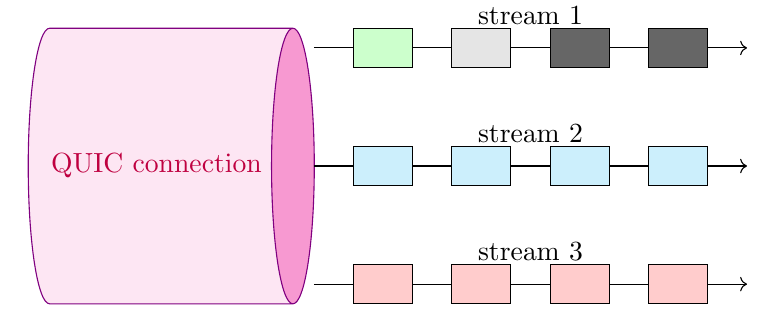
\begin{tikzpicture}

        \node[cylinder,
        draw = violet,
        text = purple,
        style={transform shape},
        cylinder uses custom fill,
        cylinder body fill = magenta!10,
        cylinder end fill = magenta!40,
        minimum size = 3.5cm] (c) at (0,0) {QUIC connection};

        \draw [->, postaction={decorate,decoration={raise=2ex, text along path,text align=center,text={stream 1}}}] (2, 1.5) -- (7.5, 1.5);
        \filldraw [fill=green!20, draw=black] (2.5, 1.25) rectangle (3.25, 1.75);
        \filldraw [fill=gray!20, draw=black] (3.75, 1.25) rectangle (4.5, 1.75);
        \filldraw [fill=black!60, draw=black] (5, 1.25) rectangle (5.75, 1.75);
        \filldraw [fill=black!60, draw=black] (6.25, 1.25) rectangle (7, 1.75);

        \draw [->, postaction={decorate,decoration={raise=2ex, text along path,text align=center,text={stream 2}}}] (2, 0) -- (7.5, 0);
        \filldraw [fill=cyan!20, draw=black] (2.5, -0.25) rectangle (3.25, 0.25);
        \filldraw [fill=cyan!20, draw=black] (3.75, -0.25) rectangle (4.5, 0.25);
        \filldraw [fill=cyan!20, draw=black] (5, -0.25) rectangle (5.75, 0.25);
        \filldraw [fill=cyan!20, draw=black] (6.25, -0.25) rectangle (7, 0.25);

        \draw [->, postaction={decorate,decoration={raise=2ex, text along path,text align=center,text={stream 3}}}] (2, -1.5) -- (7.5, -1.5);
        \filldraw [fill=red!20, draw=black] (2.5, -1.75) rectangle (3.25, -1.25);
        \filldraw [fill=red!20, draw=black] (3.75, -1.75) rectangle (4.5, -1.25);
        \filldraw [fill=red!20, draw=black] (5, -1.75) rectangle (5.75, -1.25);
        \filldraw [fill=red!20, draw=black] (6.25, -1.75) rectangle (7, -1.25);


    \end{tikzpicture}
    \caption{Stream multiplexing in a single QUIC connection}
    \label{fig:stream-multiplexing}
\end{figure}


\section{Flow control}
\label{sec:flow-control-and-congestion-control}
Flow control is a mechanism which allows receiver to announce how much data it is able to process/buffer and sender must
not exceed this limit until it is updated.
In QUIC, flow control limits can be set on two levels.
The first one is stream level -- it is set per stream type e.g.\ for all unidirectional streams opened by the peer or for all bidirectional streams opened locally.
There is no possibility to set flow control limit for a stream with a particular id.
The second one is connection level and it limits overall data amount that can be sent within the whole connection across all streams.
QUIC allows also for limiting number of streams that can be opened by the peer.
These limits are also set per stream type -- unidirectional or bidirectional and initiated by a peer or locally.

It might look like smaller granulation of flow control configuration (setting flow control limit per stream instead of
stream type) could provide more flexibility and could fit better in different use cases but similar mechanism can
be achieved using stream prioritization in the way described above (see section~\ref{sec:streams}).


\section{Congestion control}
\label{sec:congestion-control}
Congestion control also limits amount of data that can be transmitted by a sender but instead of protecting receiver it aims to prevent
from overwhelming network middleboxes like routers and if such overwhelm occurs it helps to recover from it.
RFC 9001~\cite{rfc9001} describes in details sender-side QUIC congestion controller similar to TCP NewReno.
It is triggered when one of QUIC packets is lost or when sender receives IP packet with ECN-CE flag set.
ECN stands for Explicit Congestion Notification while CE stand for Congestion Experienced and it is a codepoint (0x11) set as
value of two least significant bits of the ToS (Type of Service) field in IP header.
Whenever some middlebox is going to be overwhelmed it sets this flag in packets that it routes from a sender to a receiver.
Receiver then informs sender that the network is overwhelmed also by sending IP packets with ECN-CE flag set.

Besides NewReno QUIC can use any other congestion control algorithm that meets requirements defined in section 3.1 of RFC 8085~\cite{rfc8085}.
This makes QUIC congestion control mechanism pluggable and allows for adapting congestion control algorithm to specific use case.


\section{Reliability}
\label{sec:reliability}
QUIC is a reliable protocol which means it guarantees delivery of each packet sent by the endpoint.
Packets are delivered to the application layer in the order they were sent.
However, there are different IETF drafts that expand QUIC with new features.
One of them called \textit{An Unreliable Datagram Extension to QUIC}\cite{bider-ssh-quic-09} allows for sending unreliable messages over QUIC\@.
This can take place in simultaneously to the reliable communication.
Unreliable messages are not subject to flow control mechanisms however, they are congestion controlled.
Each unreliable message is also acknowledged so that application layer can be provided with the packet loss information.
Section~\ref{sec:partial-reliability} describes Datagram extension in details.


\section{Other transport protocols}
\label{sec:other-transport-protocols}
This section compares QUIC with three main transport protocols -- TCP, UDP and SCTP\@.

\subsection{TCP}
\label{subsec:tcp}
Transmission Control Protocol -- connection-oriented, stream oriented and reliable transport protocol.
It guarantees the order of messages and provides flow control and congestion control mechanisms.
TCP is not a multiplexed protocol.
In one TCP connection we have one logical communication channel.
This is the reason of head of line blocking problem that appears when many HTTP/2 requests are multiplexed in one TCP connection.
Because of its reliability, TCP is not a good choice for many types of interactive communication.

\subsection{UDP}
\label{subsec:udp}
User Datagram Protocol -- connection less, unreliable transport protocol.
It does not ensure that messages are delivered in the same order they were sent.
Datagrams, in this protocol, are not acknowledged nor congestion controlled.
It does not also introduce any flow control mechanisms.
Thanks to its simplicity and low bandwidth affection it is the base for RTP protocol which is widely used for transmitting multimedia.
Unlike TCP, UDP also allows for multicast transmission.
However, multicast is rarely used, mostly in local networks.

\subsection{SCTP}
\label{subsec:sctp}
Stream Control Transmission Protocol -- reliable, message oriented transport protocol.
Messages in SCTP can be delivered in order or out of order which is indicated by \textit{U} flag in DATA chunk.
DATA chunk can be thought as similar entity to QUIC frame and it can contain either control information or user data.
Chunks with \textit{U} flag set to 1 are immediately conveyed to the upper layer.
In particular setting \textit{U} flag to 1 for each DATA chunk makes whole communication unordered.
Unlike TCP and similarly to QUIC, SCTP is multistream protocol -- it allows for opening multiple logical streams in one physical connection.
Another feature of SCTP is multi-homing in which an endpoint uses two different addresses introducing some kind of fault tolerance --
one address is designated as a primary and the other one can be used in case of failure of the first one.
SCTP operates on connection less packet network such as IP therefore it needs dedicated support in middleboxes so that they can
recognize its packets correctly.
Lack of this support led to the fact that SCTP was not implemented on a mass scale and its main domain is telecommunication.
This is something that QUIC does not repeat as QUIC packets are seen by routers as usual UDP datagrams.

\subsection{Summary}
\label{subsec:summary}
Table~\ref{tab:protocols_comparision} presents a short summary of transport protocols comparison.
\begin{table}[h]
    \centering
    \resizebox{\columnwidth}{!}{%
    \begin{tabular}{|c | c | c | c | c |}
        \hline
        & TCP           & UDP              & SCTP                                   & QUIC                           \\
        \hline
        reliability        & reliable      & unreliable       & unreliable/partially reliable/reliable & unreliable/reliable            \\
        \hline
        transmission       & byte oriented & message oriented & message oriented                       & message oriented/byte oriented \\
        \hline
        flow control       & yes           & no               & yes                                    & only for streams               \\
        \hline
        congestion control & yes           & no               & yes                                    & yes                            \\
        \hline
        packets order      & ordered       & unordered        & unordered/partially ordered/ordered    & unordered/ordered              \\
        \hline
        multistream        & no            & no               & yes                                    & yes                            \\
        \hline
    \end{tabular}%
    }
    \caption{\label{tab:protocols_comparision}Transport protocols comparison.}
\end{table}

    \clearpage
    \section{State of the art}
\label{sec:state-of-the-art}

The number of QUIC publications at the moment of writing this thesis is limited.
The main reason of such situation is that QUIC was standardize just a few months ago.
In this section I present an overview of publications that are important in terms of current main QUIC usage which is
HTTP/3, are somehow related to transporting media over QUIC or are dedicated to aspects that are also important
in interactive communication.

\textit{The QUIC Fix for Optimal Video Streaming} article~\cite{the-quic-fix-for-optimal-video-streaming} introduces unreliable data transmission over QUIC and presents how combination of reliable and unreliable transmission fares in video streaming and outperforms TCP and reliable mode of QUIC\@.
Authors of this document tag H.264 video frames depending on their importance.
\textit{I-Frames} which are independent frames meaning they can be displayed without any additional frames are marked to be sent reliably.
\textit{P-Frames} which are much smaller in size and code only the difference between \textit{I-Frame} and the next frame are marked to be sent unreliably.
The same approach is applied to \textit{B-Frames} that depends on both \textit{I-Frames} and \textit{P-frames}.
Authors state that the loss of \textit{P-Frames} or \textit{B-Frames} has minimal or no impact on the user's quality of experience (QoE).
They use i.a. \textit{buffering ratio (bufRatio)} and \textit{rate of buffering (rateBuf)} metrics to measure the difference in performance of streaming video over codec-agnostic DASH protocol used with TCP, traditional QUIC and QUIC with addition of unreliable transmission.
\textit{BufRatio} is the amount of time spent on re-buffering video comparing to the total video duration, represented as a percentage.
\textit{RateBuf} is the frequency of the buffering events~\cite{impact-of-video-quality-on-user-engagement}.
As a result, \textit{bufRatio}, with packet loss set to 0.64\%, for TCP is 105\%, for QUIC is 30\% and for QUIC with addition of unreliable data transmission is less than 1\%.
\textit{RateBuf}, with the same packet loss, is equal to 50\% for TCP, 19\% for QUIC and nearly 0\% for QUIC with addition of unreliable data transmission.

\textit{QUIC: Better for what and for whom?} article~\cite{quic-better-for-what-and-for-whom} compares the page load time (PLT) for HTTP/2 requests over QUIC and TCP/TLS in different network conditions and architectures as well as for different website complexities.
Authors prepared both local and remote testbeds.
In the remote one client's machine is connected to the Internet over ADSL (to router over Ethernet or Wi-Fi) or 4G\@.
Different network conditions mean different packet loss rate and delay.
In case of complexity of site there is Youtube service in which different resources might be distributed over many servers and Doctor (website of the ANR project) website where ale files are located on the same server.
Authors concludes that QUIC outperforms HTTP/2 over TCP/TLS in unstable networks but in case of stable and reliable networks the benefits of QUIC are not so obvious.

\textit{Game of protocols: Is QUIC ready for prime time streaming?} article~\cite{game-of-protocols} compares QUIC and TCP in HAS (HTTP adaptive streaming) applications.
To this end, authors performed experiments in four scenarios.
Frame-seek scenario is about seeking to the specified frame in the video.
Connection-switch scenario is about changing the connection from e.g.\ Wi-Fi to 3G\@.
Multiplexing scenario is about comparing different stream multiplexing techniques i.e.\ HTTP/1.1 over varying number of TCP connections, HTTP/2 with parallel requests over a single TCP connection and QUIC over a single UDP connection.
Fairness scenario is about checking fairness of congestion control mechanisms while there are multiple competing clients.
Authors also used three different adaptive algorithms: BASIC, SARA and BBA-2.
In the frame-seek scenario QUIC behaved better for all adaptive algorithms and types of networks reducing numerically \textit{rebufferRate} metric (which is a similar metric to \textit{bufRatio}) by 1--3\%.
In the WiFi-LTE and WiFi-3G connection-switch scenario, QUIC also behaved better for all adaptive algorithms reducing numerically \textit{rebufferRate} by 1\% for SARA and BBA-2 and by 7\% for BASIC\@.
Evaluation of different multiplexing techniques showed that in the typical network conditions all three methods resulted in the similar average playback bitrate.
In the large delay and typical loss network, QUIC performed best.
For typical delay and large loss as well as for large delay and large loss, HTTP/1.1 with varying number of TCP connections was better than QUIC\@.
HTTP/2 over single TCP connection didn't manage to beat any of the other multiplexing techniques in any of the network conditions.
Fairness examination of congestion control mechanisms in TCP and QUIC showed that for typical packet loss and delay both protocols guarantee fair resource access for competing clients which results in the similar average playback bitrate.
In the large loss scenario single QUIC client was able to achieve higher bitrate (about 37\%) than single TCP client.
For competing clients, QUIC still was able to achieve better bitrate than TCP (about 40\%).
In the large delay scenario, the results were similar to the large loss scenario.
The last one scenario with large loss and large delay showed that TCP client was able to achieve higher bitrate (about 16\%) both when competing and not competing with QUIC client.

\textit{And QUIC meets IoT: performance assessment of MQTT over QUIC} article~\cite{and-quic-meets-iot} maps MQTT to QUIC
and compares its performance with state-of-the-art MQTT over TCP\@.
Authors performed two tests.
In the first one, they send 1000 MQTT messages to the broker which then are sent to the subscriber.
In the second one, they establish MQTT connection and send only one message and close the connection.
The purpose of the second scenario was to see improvements introduced by QUIC in terms of faster connection establishment.
Both tests were performed in three different, emulated network environments: Wi-Fi, 4G/LTE and Satellite.
Authors states that MQTT over QUIC outperforms MQTT over TCP however, they expected a bigger advantage
of QUIC in the second scenario due to QUIC 0-RTT packets.

\textit{Emerging Interactive Applications over QUIC} article~\cite{9045245} compares QUIC performance with TCP and UDP
using three multimedia services.
The first service which is cloud gaming represents an interactive communication.
The second and third ones which are 4K video streaming and client-server online gaming represent classic multimedia
applications.
Each client in each service was connected to the Access Point which had access to the Internet.
The bottle neck was the connection between AP and router to which three servers (one for each service) were connected.
The first experiment tests QUIC fairness and shows that average achieved bandwidth by Cloud Gaming and 4K streaming
is more balanced when using QUIC\@.
The second experiment tests QUIC end-to-end latency and shows a significant delay reduction for all three services when using QUIC\@.
In the last scenario, authors compare Round Trip Time when streaming 4K video using QUIC and TCP\@.
Experiment shows that RTT for QUIC is lower than for TCP\@.
To sum up in all scenarios QUIC outperforms traditional transport protocols both for interactive and classic multimedia
applications.

\textit{Media QoE Enhancement With QUIC} article~\cite{7562075} uses QUIC stream prioritization to improve Quality of Experience (QoE).
Authors focus on MPEG-DASH based application.
They prioritize streams that carry multimedia data depending on the client's player buffer.
If its level is below 20 sec then client requests subsequent media chunks with high priority.
For buffer level between 20 and 80 sec medium priority is requested and for buffer level above 80 sec high priority.
The experiment shows that stream prioritization gain in Initial Buffering Time can be from 6\% to 49\% depending on
bandwidth limit and video resolution.
%
%\textit{Impact of ACK Scaling Policies on QUIC Performance} article~\cite{9524947}
%
%
%
%\textit{An attempt at introducing Multipath in QUIC} article~\cite{8806051}

%\textit{A Pure HTTP/3 Alternative to MQTT-over-QUIC in Resource-Constrained IoT} article~\cite{iot} compares performance
%of public-subscribe architecture realized with HTTP/3 over QUIC and MQTT over QUIC\@.

    \clearpage
    %! suppress = EscapeAmpersand


\section{Evaluation}
\label{sec:evaluation}

%\subsection{QUIC and HTTP/3}
%\label{subsec:quic-and-http/3}

\subsection{Hello world application}
\label{subsec:hellow-world-application}
QUIC is a user level protocol which means there is no need to recompile operating system kernel to provide it with support
for QUIC\@.
The most popular implementations of QUIC at the moment of writing this thesis are those written in Rust and Go.
However there are plenty of other implementations e.g.\ in C, Java or C++.

\subsubsection{Importing QUIC in a project}
Importing QUIC in a project depends on used language and is as easy as importing any other dependency.
In Rust it is done simply by putting \lstinline{"quiche=0.10.0"} in \textit{Cargo.toml}.
In C user has to compile QUIC library as a static or dynamic one and include it in its \textit{Makefile}, \textit{CMakeLists.txt}
or any other build tool.

\subsubsection{Libraries architecture}
In my thesis I was mostly using two implementations -- \textit{quiche} which is written in Rust and \textit{lsquic} which is written in C\@.
The way both libraries work is presented in figure~\ref{fig:quic-implementations-architecture}.
\begin{figure}
    \centering
    \tikzstyle{rect}=[rectangle,minimum width=2cm,minimum height=2cm,draw=black]
    \begin{tikzpicture}[node distance=2cm]
        \node[rect,align=center] (quic-library) {QUIC\\library};

        \node[rect,align=center,right=of quic-library] (server-side) {server\\side}
        edge [<-,bend right] node[above,align=center] {QUIC\\packets} (quic-library)
        edge [->,bend left] node[align=center,below] {QUIC\\packets} (quic-library);
        \node[rectangle,draw=black,above=of server-side.south] (server-socket) {sock};

        \node[rect,align=center,left=of quic-library] (quic-library-2) {QUIC\\library};
        \node[rect,align=center,left=of quic-library-2] (client-side) {client\\side}
        edge [<-,bend right] node[below,align=center] {QUIC\\packets} (quic-library-2)
        edge [->,bend left] node[align=center,above] {QUIC\\packet} (quic-library-2);
        \node[rectangle,draw=black,above=of client-side.south] (client-socket) {sock};

        \draw[<->,bend left] (client-socket.north) to node[align=center,above] {QUIC packets} (server-socket.north);
    \end{tikzpicture}
    \caption{Architecture of QUIC implementations}
    \label{fig:quic-implementations-architecture}
\end{figure}
Both quiche and lsquic are used to generate QUIC packets that has to be transmitted to the other side.
This transmission is left to the user.
None of libraries manages UDP socket for the user.
QUIC packets are generated whenever user sends some data, receives some data or connection timeout expires.
This approach has one advantage -- user can use its own UDP socket which can be helpful when integrating QUIC
with some other already existing systems.
On the other hand user has to exactly know when to call which functions.
For example whenever some QUIC packets are received from the network and passed to the QUIC engine
user has to call function that will generate some QUIC control packets like those containing ACK frames
and has to send them to the peer.
Calling functions at a wrong moment (too late) can result in some misbehaviour of QUIC engine (e.g.\
we can receive some more packets due to not sending acknowledgments in a proper time).

\FloatBarrier

\subsubsection{Example usage}
Following listing presents simplified example usage of quiche library.
It is taken from quiche repository.
\begin{lstlisting}[label={lst:lstlisting2},caption={Simplified example usage of quiche library.},captionpos=b]
loop {
    poll.poll(&mut events, conn.timeout()).unwrap();

    loop {
        // if there are no events it means
        // that timer has expired - handle it and
        // break reading loop
        if events.is_empty() {
            conn.on_timeout();
            break;
        }

        // read data from UDP socket
        let read = socket.recv_from(&mut buf);
        if read == 0 {
            break;
        }

        // process potentially coalesced packets
        conn.recv(&mut buf).unwrap();
    }

    // send actual data
    if conn.is_established() && !req_sent {
        conn.stream_send(req);
        req_sent = true;
    }

    // check wheather there is any data
    // in any stream for the user
    for stream in conn.readable() {
        conn.stream_recv(stream, &mut buf);
        print!("Got data: {}", buf);
    }

    // generate outgoing QUIC packets
    // and send them on UDP socket
    loop {
        let written = conn.send(&mut out);
        if written == 0 {
            break;
        }
        socket.send(&out);
    }
}
\end{lstlisting}

There is one main loop which consists of three more loops.
The first one is responsible for reading data from socket and feeding it to the quiche.
If there is no data to read but connection timer has expired then \lstinline{conn.on_timeout()} has to be called.
After calling \lstinline{conn.on_timeout()} next call to \lstinline{conn.send()} will generate some QUIC control packets.
The second loop is responsible for generating quic packets using \lstinline{conn.send()} and sending them through on
the UDP socket.
There is also a \textit{for} loop that is responsible for checking if we received any data on any stream

\subsubsection{Summary}
QUIC libraries can be very easily imported into any environment.
However some of them like quiche may require from a user more awareness what needs to be done e.g.\
when to call \lstinline{conn.on_timeout()} or \lstinline{conn.send()} functions.
On the other hand leaving managing the socket to the user guarantees more flexibility and allows for easier integration with
other protocols or standards.

\clearpage

\subsection{Packet encryption overhead}
\label{subsec:packet-encryption-overhead}
This section outlines QUIC encryption process and compares its performance with SRTP encryption process.
I chose SRTP to compare QUIC with as it is used for carrying multimedia data and it includes similar data in its
header as QUIC does.
Similar performance of encryption process in both protocols is promising and allows for further research in topic
whether RTP can be replaced by QUIC in some scenarios.
Such a replacement can significantly reduce complexity of already existing systems and standards which I am describing
more in section~\ref{subsec:webrtc-over-quic}.

\subsubsection{QUIC payload encryption}
Payload is encrypted using AEAD algorithm.
All cipher-suites used in TLS 1.3 are allowed in QUIC except \textit{AES\_128\_CCM\_8}.
Therefore we have \textit{AES\_128\_GCM}, \textit{AES\_256\_GCM}, \textit{CHACHA20\_POLY1305} and \textit{AES\_128\_CCM}.
Figure~\ref{fig:payload_enc} shows the process of payload encryption.
As a plain text we pass payload and as an associated data we pass plain header.
As a result we get a ciphertext and an authentication tag.

\begin{figure}[h]
    \centering
    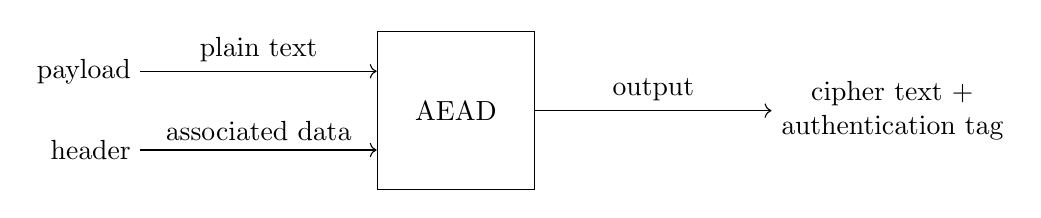
\begin{tikzpicture}
        \node (aead) [rectangle, draw=black, minimum width=2cm,minimum height=2cm] {AEAD};
        \node (aead in 0) [rectangle, minimum width=1cm,minimum height=1cm, above left=of aead.south east] {};
        \node (aead in 1) [rectangle, minimum width=1cm,minimum height=1cm, below left=of aead.north east] {};
        \node (payload) [left=3cm of aead in 0] {payload}
        edge [->] node[align=center,above] {plain text} (aead in 0);
        \node (header) [left=3cm of aead in 1] {header}
        edge [->] node[align=center,above] {associated data} (aead in 1);
        \node (cipher text) [align=center, right=3cm of aead] {cipher text + \\ authentication tag}
        edge [<-] node[align=center, above] {output} (aead);
    \end{tikzpicture}
    \caption{QUIC payload encryption scheme}
    \label{fig:payload_enc}
\end{figure}

\subsubsection{QUIC header encryption}
Figure~\ref{fig:header_enc} shows the process of header encryption.
The first step is to get \textit{sample} from encrypted payload.
In most cases a sample is 16 bytes long and it is taken starting from $4 - pn\_len$ byte of encrypted payload.
In the next step the sample is encrypted and its first 5 bytes are taken as mask.
At the end we perform XOR operation on predefined header fields and mask.
As a result we get header with some fields being encrypted.
Algorithm used to encrypt sample depends on negotiated cipher-suite.
For example, if payload is encrypted with AES\_128\_GCM then sample will be encrypted using AES\_128\_ECB\@.

\begin{figure}[h]
    \centering
    \tikzset{XOR/.style={draw,circle, minimum width=1cm, minimum height=1cm, append after command={
    [shorten >=\pgflinewidth, shorten <=\pgflinewidth,]
    (\tikzlastnode.north) edge (\tikzlastnode.south)
    (\tikzlastnode.east) edge (\tikzlastnode.west)}}}
    \begin{tikzpicture}
        \node (xor) [XOR, scale=1.2] {};
        \node (encrypted header) [right=of xor] {encrypted header}
        edge [<-] node[align=center,above] {} (xor);
        \node (mask) [below left=of xor] {mask}
        edge [->, to path={-| (\tikztotarget)}] (xor.south);
        \node (sample) [left=of mask] {sample}
        edge [->] (mask);
        \node (payload) [left=of sample] {payload}
        edge [->] (sample);
        \node (header)  at (payload |- xor) {header}
        edge [->] (xor);
    \end{tikzpicture}
    \caption{QUIC header encryption scheme}
    \label{fig:header_enc}
\end{figure}

\subsubsection{RTP packet encryption}
Encryption of RTP packets is specified by extension to RTP protocol called SRTP (RFC 3711~\cite{rfc3711}).
SRTP protects only RTP payload and leaves RTP header unencrypted.
SRTP uses AES cipher in two modes f8-mode or Counter Mode.
The following tests compares the performance of both encryption mechanisms using AES\_128\_GCM\@.

\subsubsection{Tests}
\label{subsubsec:tests}
Following tests are split into two scenarios.

In the first one I am comparing time needed for encrypting constant length QUIC header (22 bytes) and variable length QUIC payload.
QUIC payload encapsulates RTP packet.
Therefore it consists of constant length flow identifier (1 byte), constant length RTP header (12 bytes) and variable length RTP payload (from 100 to 1200 bytes).

In the second scenario I am comparing time needed for encrypting standalone variable length RTP payload (from 100 to 1200 bytes)
and whole QUIC packet which consists of constant length QUIC header (22 bytes) and variable length QUIC payload.
QUIC payload has the same format as in the first test scenario.
Whole QUIC packet size can be obtained from the equation~\ref{eq:quic-packet-size}.
\begin{align}
    \begin{split}
        QUIC\_packet\_size & = RTP\_payload\_size + RTP\_header\_size \\
        & \quad + tag\_identifier + QUIC\_header\_size \\
        & = RTP\_payload\_size + 12 + 1 + 22 \\
        & = RTP\_payload\_size + 35
    \end{split}
    \label{eq:quic-packet-size}
\end{align}

In both test scenarios, encryption process was performed concurrently.

\subsubsection{Environment}
Test environment:
\begin{itemize}
    \item processor: Intel(R) Core(TM) i5-9600K CPU @ 3.70GHz, 6 Cores, 9 MB Cache
    \item memory: 16 GB RAM
    \item operating system: Linux
    \item library: ring 0.16.20
    \item language: Rust
    \item cipher-suite: AES\_128\_GCM
\end{itemize}

\subsubsection{Methodology}
For each RTP payload size following steps were performed:
\begin{itemize}
    \item collect 100 samples
    \item detect and remove outliers
    \item count average from remaining samples
\end{itemize}

\subsubsection{Results}
Figure~\ref{fig:header-payload-enc} presents time comparison between header and payload encryption process.
We can see that QUIC payload encryption time is between 220 and 450 ns.
For 400, 800 and 1200 RTP payload sizes we can observe shorter encryption time than for previous sizes.
This is probably because of concurrent execution of encryption process.
The data can be split across threads in a manner that allocates additional thread for 400, 800 and 1200 bytes.

\begin{figure}[h]
    \centering
    \begin{tikzpicture}
        \begin{axis}[xlabel={RTP payload size (bytes)},
        ylabel={Average time (ns)},
        legend style={legend pos=outer north east}]
            \addplot table[x=size,y=time] {data/quic-header-enc.table};
            \addlegendentry{Header encryption time}
            \addplot table[x=size,y=time] {data/quic-payload-enc.table};
            \addlegendentry{Payload encryption time}
        \end{axis}
    \end{tikzpicture}
    \caption{QUIC header vs QUIC payload encryption time}
    \label{fig:header-payload-enc}
\end{figure}

Figure~\ref{fig:rtp-payload-quic-packet-enc} presents time comparison between RTP payload and QUIC packet (with RTP packet inside) encryption process.
As in the first test scenario, for 400, 800 and 1200 RTP payload sizes we can observe shorter encryption time than for previous sizes.
Encryption of QUIC packet that encapsulates RTP packet is slower by 30--50ns comparing to standalone RTP payload encryption.
This is illustrated in figure~\ref{fig:rtp-payload-quic-packet-enc}.

\begin{figure}[!h]
    \centering
    \begin{tikzpicture}
        \begin{axis}[xlabel={RTP payload size (bytes)},
        ylabel={Average time (ns)},
        legend style={legend pos=outer north east}]
            \addplot table[x=size,y=time] {data/quic-packet-enc.table};
            \addlegendentry{QUIC packet encryption time}
            \addplot table[x=size,y=time] {data/rtp-payload-enc.table};
            \addlegendentry{RTP payload encryption time}
        \end{axis}
    \end{tikzpicture}
    \caption{RTP payload vs QUIC packet (with RTP packet inside) encryption time}
    \label{fig:rtp-payload-quic-packet-enc}
\end{figure}

In summary, QUIC header encryption does not introduce a significant overhead for the entire QUIC packet encryption process.
Also, encryption of encapsulated RTP packet into QUIC packet is insignificantly slower than encryption of standalone RTP payload.

\clearpage

\subsection{Partial reliability}
\label{subsec:partial-reliability}
QUIC is by default a reliable protocol.
However there are plenty of situations where transmission speed is more important than reliability, especially in real-time communication.
\textit{An Unreliable Datagram Extension to QUIC}~\cite{ietf-quic-datagram-02} introduces a new QUIC frame called DATAGRAM which carry data unreliably.

DATAGRAM frames are not retransmitted.
They are sent alongside the STREAM frames so they use the same cryptographic context but they do not affect flow-control limits.
Each DATAGRAM frame is acknowledged so it is possible to provide application with information about packet loss.
It is also important that DATAGRAM frames are subject to QUIC congestion control mechanism which allows applications to avoid implementing their own.

Two experiments have been performed to validate DATAGRAM frames behavior as well as their ease of use.
They are presented in the following sections.

\subsubsection{QUIC flow control}
\label{subsubsec:quic-flow-control}
As stated in section~\ref{subsec:flow-control-and-congestion-control} there are two levels of flow control in QUIC -- stream level and connection level.
Initial limits are set by the receiver in transport parameters during QUIC handshake.
Subsequent updates are done by sending \\ \textit{MAX\_STREAM\_DATA} or \textit{MAX\_DATA} frames.
It is implementation choice when and how much increase the limit.
Frequently sending frames with small updates will result in increased bandwidth usage.
On the other hand, less frequent but larger updates require more resources at the receiver.
Sender must not exceed limits set by the receiver.
If sender is blocked in transmitting data it should send \textit{STREAM\_DATA\_BLOCKED} or \textit{DATA\_BLOCKED} frames.
Flow control mechanism is described in details in section 4, RFC 9000~\cite{rfc9000}.

DATAGRAM frames are not subject to QUIC flow control mechanism.
This can be useful especially in scenarios where we are sending both reliable and unreliable data.
If reliable data are not crucial (e.g.\ uploading or downloading a file from a chat) its transmission can be limited in favour of unreliable data (e.g.\ voice or video).

\subsubsection{QUIC loss detection}
\label{subsubsec:loss-detection}
From RFC 9002 (Section 6.1), a packet is declared lost if it meets all of the following conditions:
\begin{itemize}
    \item The packet is unacknowledged, in flight, and was sent prior to an acknowledged packet.
    \item The packet was sent kPacketThreshold packets before an acknowledged packet (Section 6.1.1), or it was sent long enough in the past (Section 6.1.2)~\cite{rfc9002}.
\end{itemize}

To consider packet is lost there has to be some other packet that was sent later and has already been acknowledged.

To this end QUIC introduces a Probe Timeout (PTO).
The Probe Timeout (PTO) triggers the sending of one or two probe datagrams when ack-eliciting packets are not acknowledged within the expected period of time or the server may not have validated the client's address.
The PTO enables a connection to recover from loss of tail packets or acknowledgments~\cite{rfc9002} (RFC 9002, Section 6.2).

Expiration of PTO timer does not indicate the packet was lost.
It only provides one of the requirements necessary to consider the packet as lost -- the packet was sent prior to an acknowledged packet.
PTO timer is reset each time a new ack-eliciting packet was sent or received.

\subsubsection{Tests}
\label{subsubsec:tests2}
Following tests are split into two scenarios.

In the first one I am presenting behaviour of DATAGRAM frames in case of reaching flow control limits on any of streams used in the connection.
In this scenario client opens two bidirectional streams while the server sets flow control limit on each of them to 1000B\@.
In each iteration client tries to send 10 reliable and 10 unreliable messages of size 800B each.

In the second one I am testing if acknowledgments of DATAGRAM frames can introduce a significant overhead to the bandwidth usage.
In this scenario client machine had configured a packet loss from 0\% to 30\% for all UDP datagrams which destination port was equal to 4433.
Packet loss was set using Linux TC software.
For each packet loss (0\%, 10\%, 30\%) client was trying to send 1000 messages of 500B size each.
Server responsibility was to respond for each message by returning it back to the client.
After sending each message client was waiting for the response from the sever specified amount of time.

\subsubsection{Environment}
\label{subsubsec:test-env}
Figure~\ref{fig:dgram-test-env} shows test environment used in DATAGRAM frames experiments.
Both machines are in local network.

\begin{figure}[h]
    \centering
    \begin{tikzpicture}[node distance = 6cm]
        \node (pc a) [anchor=west,align=center,label=below:{Server}] {\includegraphics{cisco_icons/workstation.eps}}
        ;
        \node (pc b) [right=of pc a,align=center,label=below:{Client}] {\includegraphics{cisco_icons/workstation.eps}}
        edge [<->] node {} (pc a);
    \end{tikzpicture}
    \caption{DATAGRAM frames test environment}
    \label{fig:dgram-test-env}
\end{figure}

\subsubsection{Results}
Figure~\ref{fig:dgram_flow_control} presents results for the first test scenario.


\begin{figure}[h]
    \centering
    \begin{sequencediagram}
        \newinst{client}{Client}
        \newinst[8]{server}{Server}
        \mess{client}{crypto,initial: 1}{server}
        \mess{server}{initial: 0,ack 1, crypto}{client}
        \mess{server}{handshake: 0,crypto}{client}
        \mess{server}{handshake: 1,crypto}{client}
        \mess{client}{ack 0,initial: 2}{server}
        \mess{client}{crypto,ack 0--1,handshake: 0}{server}
        \mess{client}{dgram,stream 0 blocked,stream 4 blocked, 1RTT: 0}{server}
        \mess{client}{stream 0,1RTT: 1}{server}
        \mess{client}{datagram,1RTT: 2}{server}
        \mess{client}{stream 4,1RTT: 3}{server}
        \mess{client}{datagram,1RTT: 4}{server}
        \mess{client}{datagram,1RTT: 5}{server}
        \mess{client}{datagram,1RTT: 6}{server}
    \end{sequencediagram}
    \caption{DATAGRAM flow control test -- sequence diagram}
    \label{fig:dgram_flow_control}
\end{figure}


%\begin{figure}
%    \centering
%    \includegraphics[width=\textwidth]{img/__09__datagrams/dgram_flow_control.png}
%    \caption{DATAGRAM flow control test -- sequence diagram}
%    \label{fig:dgram_flow_control}
%\end{figure}

After establishing the connection client starts sending data.
It sends two 1-RTT packets with STREAM frames (packets 1 and 3) and reaches flow control limit.
However, he is still able to send packets with DATAGRAM frames (packets 4, 5, 6).

%Figure~\ref{fig:dgram_flow_control2} shows this behavior from different perspective.
%\begin{figure}
%    \centering
%    \includegraphics[width=\textwidth]{img/__09__datagrams/dgram_flow_control_2.png}
%    \caption{DATAGRAM flow control test -- limits}
%    \label{fig:dgram_flow_control2}
%\end{figure}
%Pink line indicates sum of stream flow control limit whereas blue bars represent data sent.
%We can see that despite the fact flow control limit is less than 5kB we send much more data -- over 45kB\@.

Table~\ref{tab:dgram_packet_loss} illustrates results for the second test scenario.

\begin{table}[h]
    \centering
    \resizebox{\columnwidth}{!}{%
    \begin{tabular}{|c | c | c | c | c | c |}
        \hline
        \multicolumn{2}{|c}{\makecell{0\% packet loss}} & \multicolumn{2}{|c}{\makecell{10\% packet loss}} & \multicolumn{2}{|c|}{\makecell{30\% packet loss}} \\
        \hline
        \multicolumn{2}{|c}{client} & \multicolumn{2}{|c|}{client} & \multicolumn{2}{|c|}{client} \\
        \hline
        packets sent & packets lost & packets sent & packets lost & packets sent & packets lost \\
        \hline
        1005         & 0            & 1007         & 89           & 1031         & 318          \\
        \hline
    \end{tabular}%
    }
    \caption{\label{tab:dgram_packet_loss}Number of packets sent with and without packet loss for DATAGRAM frames.}
\end{table}

For packet loss set to 0\% client sent 1005 packets.
None of them were lost.
5 additional packets comes from handshake establishment.
In this setup QUIC didn't send any additional packets acknowledging DATAGRAM frames.

For packet loss set to 10\% client sent 1007 packets, 89 of which were lost.
We can see that in this configuration client sent 2 packets more than previously.
This is because server sends its data as last and client need to acknowledge this data by sending additional packet with ACK frame.

For packet loss set to 30\% client sent 1031 packets, 318 of which were lost.
This time we can observe that client sent 20--30 packets more than in the first two scenarios.
It's because of PING frames that are being sent when PTO timer expires.
Figure~\ref{fig:dgram_ping_frames} illustrates this situation.

\begin{figure}[h]
    \centering
    \begin{sequencediagram}
        \newinst{client}{Client}
        \newinst[8]{server}{Server}
        \mess{client}{datagram,ack 27,1RTT: 36}{server}
        \mess{server}{1RTT: 28,ack 36, datagram}{client}
        \mess{client}{datagram,ack 28,1RTT: 37}{server}
        \mess{server}{1RTT: 29,ack 36, ping}{client}
        \mess{client}{datagram,ack 28--29,1RTT: 38}{server}
        \mess{client}{ping,ack 28--29,1RTT: 39}{server}
    \end{sequencediagram}
    \caption{Additional PING frames after server or client inactivity}
    \label{fig:dgram_ping_frames}
\end{figure}

%\begin{figure}
%    \centering
%    \includegraphics[width=\textwidth]{img/__09__datagrams/dgram_retransmission_ping.png}
%    \caption{Additional PING frames after server or client inactivity}
%    \label{fig:dgram_ping_frames}
%\end{figure}

Server in its 28th 1RTT packet sent datagram frame in response to client's earlier packet and set its PTO timer.
Client received server's packet, generated a response and set its own timer.
The response was lost so that server's PTO timer expired which resulted in 29th 1RTT packet from server to client with PING frame.
After receiving it client generated a response, reset its PTO timer and sent the response but this time it was also lost.
After 21 ms client's PTO timer expired so client sent a new ack-eliciting packet with PING frame.

In summary, a small overhead related to acknowledging DATAGRAM frames was observed for network environment with a very
high packet loss (30\%).
In other scenarios -- when there was no packet loss or packet loss was equal to 10\% acknowledging DATAGRAM frames
did not introduce any overhead to the connection bandwidth.

\clearpage

\subsection{Video over QUIC}
\label{subsec:video}
This section outlines \textit{video\_quic} application which I developed to observer how QUIC behave when used for
sending multimedia data.
\textit{video\_quic} sends H264 encoded video from a client to a server.
It is written in Elixir and uses Membrane Framework and quicer library.
%Membrane Framework is a framework for processing multimedia in Elixir while quic is a library that
%brings QUIC to the Elixir World.
%quic is a wrapper around another library called msquic.
%Both in Elixir and Erlang there is a possibility to define function and implement its body in C language.
%quic uses this feature to define QUIC API in Erlang and provide implementation in C.
%This implementation just calls functions from msquic which is an actual implementation of QUIC written in C.

\subsubsection{quicer}
quicer is a library written in Erlang which brings QUIC to the Erlang ecosystem.
It provides NIF bindings for another library called msquic which is actual implementation of QUIC written in C\@.
NIF stands for Native Implemented Function and it allows for combining C and Erlang code.
NIFs are functions declared in Erlang but their implementations are provided in C\@.
They are called in the same way as any other Erlang functions.
%To serialize and deserialize arguments between Erlang and C code \textit{erl\_nif} library has to be used.
quicer can be thought as a wrapper around actual QUIC implementation.
Even though at the moment of writing this thesis quicer lacked support for DATAGRAM frames.
To implement video\_quic I had to add support for DATAGRAMS in quicer by wrapping proper functions from msquic.
Those changes are available publicly on GitHub\footnote{\url{https://github.com/emqx/quic/pull/57}}.

\subsubsection{Membrane Framework}
Membrane Framework is a framework for processing multimedia in Elixir.
The most elementary entity in Membrane is an element.
There are four types of elements.
\begin{description}
    \item [Source] - elements of type source are responsible for reading data from a disk or network and passing them to
    other Membrane elements.
    \item [Filter] - it receives data from other Membrane elements (sources and filters), processes this data and passes
    modified (or the same) data to next Membrane elements
    \item [Sink] - elements of this type are something opposite to sources.
    They receive data from other Membrane elements and save it to a file or send it through a network.
    \item [Bin] - it is used only for logical purposes particularly it is used for grouping multiple Membrane elements into one.
    Bin does not modify, read or send data.
\end{description}
Membrane elements are linked together into Pipelines.
Pipeline can be thought as a unidirectional flow of data.

Figure~\ref{fig:example-membrane-pipeline} presents a very simple Membrane pipeline that is responsible for reading
MP3 audio file and playing it in headphones.
In this example there is the MP3 File Reader which reads data and passes it to the MP3 Decoder.
MP3 Decoder decodes each chunk of data and passes it to the Converter.
Converter prepares each chunk of audio for playing it and passes it to PortAudio which then plays it in headphones.
\begin{figure}[h]
    \centering
    \tikzstyle{rect}=[rectangle,minimum width=2cm,minimum height=2cm,draw=black]
    \scalebox{0.9}{%
    \begin{tikzpicture}
        \node[label=below:{MP3 audio file}](file){
        \begin{tikzpicture}
            \draw (0,0) -- (0,1.2) -- (0.7,1.2) -- (0.7,0.8) -- (1,0.8) -- (1,0) -- cycle;
            \draw (0.7,1.2) -- (1,0.8);
            \foreach \y in {0.2,0.4,0.6}{
            \draw (0.2,\y) -- (0.8,\y);
            \draw (0.2,0.8) -- (0.6,0.8);
            \draw (0.2,1) -- (0.6,1);
            }
        \end{tikzpicture}
        };
        \node[rect,fill=cyan!30,right=of file,align=center] (file-src) {MP3 File \\ Reader \\ (Source)}
        edge [<-] node[align=center,right] {} (file);
        \node[rect,fill=purple!30,right=of file-src,align=center] (mp3-decoder) {MP3 \\ Decoder \\ (Filter)}
        edge [<-] node[align=center,right] {} (file-src);
        \node[rect,fill=purple!30,right=of mp3-decoder,align=center] (converter) {Converter \\ (Filter)}
        edge [<-] node[align=center,right] {} (mp3-decoder);
        \node[rect,fill=green!30,right=of converter,align=center] (port-audio) {PortAudio \\ (Sink)}
        edge [<-] node[align=center,right] {} (converter);
    \end{tikzpicture}%
    }
    \caption{Example Membrane Pipeline}
    \label{fig:example-membrane-pipeline}
\end{figure}

To use Membrane I implemented two new Membrane elements -- QUIC Sink and QUIC Source.
They are also available publicly on GitHub\footnote{\url{https://github.com/mickel8/membrane_quic_plugin}}.
Both of them use quicer -- QUIC Source for sending data and QUIC Sink for receiving data through the network.

\subsubsection{Architecture}
\label{subsubsec:architecture}

Figure~\ref{fig:video-app-architecture} illustrates architecture of video quic application.
It consists of two pipelines.
Client pipeline is responsible for reading data from a file and sending it through the network while the server one is
listening on a connection and after receiving any data it decodes this data and play it using SDL player.
Architecture of both pipelines is presented in figure~\ref{fig:pipelines}.

\begin{figure}[h]
    \centering
    \tikzstyle{rect}=[rectangle,minimum width=2cm,minimum height=2cm,draw=black]
    \begin{tikzpicture}
        \node[label=below:{H264 video file}](file){
        \begin{tikzpicture}
            \draw (0,0) -- (0,1.2) -- (0.7,1.2) -- (0.7,0.8) -- (1,0.8) -- (1,0) -- cycle;
            \draw (0.7,1.2) -- (1,0.8);
            \foreach \y in {0.2,0.4,0.6}{
            \draw (0.2,\y) -- (0.8,\y);
            \draw (0.2,0.8) -- (0.6,0.8);
            \draw (0.2,1) -- (0.6,1);
            }
        \end{tikzpicture}
        };
        \node[rect,right=of file,align=center] (server-pipeline) {Client \\ side \\ pipeline}
        edge [<-] node[align=center] {} (file);
        \node[label=center:Internet,right=of file-src] (internet) {\includegraphics{cisco_icons/cloud.eps}}
        edge [<-] node[align=center] {} (server-pipeline);
        \node[rect,right=of internet,align=center] (client-pipeline) {Server \\ side \\ pipeline}
        edge [<-] node[align=center] {} (internet);
    \end{tikzpicture}
    \caption{Architecture of video quic application}
    \label{fig:video-app-architecture}
\end{figure}

\begin{figure}[h]
    \tikzstyle{rect}=[rectangle,minimum width=2cm,minimum height=2cm,draw=black]
    \subfloat[Client side pipeline]{
    \begin{tikzpicture}
        \node[rect,align=center,fill=cyan!30] (file-src) {File \\ Source};
        \node[rect,right=of file-src,align=center,fill=purple!30] (video-parser) {Video \\ Parser}
        edge [<-] node[align=center,right] {} (file-src);
        \node[rect,right=of video-parser,align=center,fill=purple!60] (rtp-session-bin) {RTP \\ Session \\ Bin}
        edge [<-] node[align=center,right] {} (video-parser);
        \node[rect,right=of rtp-session-bin,fill=purple!30] (realtimer) {Realtimer}
        edge [<-] node[align=center,right] {} (rtp-session-bin);
        \node[rect,right=of realtimer,align=center,fill=green!30] (quic-sink) {Quic \\ Client}
        edge [<-] node[align=center,right] {} (realtimer);
    \end{tikzpicture}
    } \\
    \subfloat[Server side pipeline]{
    \begin{tikzpicture}
        \node[rect,below left=of internet,align=center,fill=cyan!30] (quic-src) {Quic \\ Server};
        \node[rect,right=of quic-src,align=center,fill=purple!60] (rtp-session-bin-2) {RTP \\ Session \\ Bin}
        edge [<-] node[align=center,right] {} (quic-src);
        \node[rect,right=of rtp-session-bin-2,align=center,fill=purple!30] (video-parser-2) {Video \\ Parser}
        edge [<-] node[align=center,right] {} (rtp-session-bin-2);
        \node[rect,right=of video-parser-2,align=center,fill=purple!30] (video-decoder) {Video \\ Decoder}
        edge [<-] node[align=center,right] {} (video-parser-2);
        \node[rect,right=of video-decoder,align=center,fill=green!30] (sdl-player) {SDL \\ player}
        edge [<-] node[align=center,right] {} (video-decoder);
    \end{tikzpicture}
    }
    \caption{Architecture of video quic pipelines}
    \label{fig:pipelines}
\end{figure}


%\begin{figure}
%    \centering
%    \tikzstyle{rect}=[rectangle,minimum width=4cm,minimum height=1cm,draw=black]
%    \scalebox{.75}{%
%    \begin{tikzpicture}
%        \node[label=below:{H264 video file}](file){
%        \begin{tikzpicture}
%            \draw (0,0) -- (0,1.2) -- (0.7,1.2) -- (0.7,0.8) -- (1,0.8) -- (1,0) -- cycle;
%            \draw (0.7,1.2) -- (1,0.8);
%            \foreach \y in {0.2,0.4,0.6}{
%            \draw (0.2,\y) -- (0.8,\y);
%            \draw (0.2,0.8) -- (0.6,0.8);
%            \draw (0.2,1) -- (0.6,1);
%            }
%        \end{tikzpicture}
%        };
%        \node[rect,below=of file] (file-src) {File Source}
%        edge [<-] node[align=center,right] {} (file);
%        \node[rect,below=of file-src] (video-parser) {Video Parser}
%        edge [<-] node[align=center,right] {} (file-src);
%        \node[rect,below=of video-parser] (rtp-session-bin) {RTP Session Bin}
%        edge [<-] node[align=center,right] {} (video-parser);
%        \node[rect,below=of rtp-session-bin] (realtimer) {Realtimer}
%        edge [<-] node[align=center,right] {} (rtp-session-bin);
%        \node[rect,below=of realtimer] (quic-sink) {Quic Sink}
%        edge [<-] node[align=center,right] {} (realtimer);
%        \node[below=of quic-sink, label=center:Internet] (internet) {\includegraphics{cisco_icons/cloud.eps}}
%        edge [<-] node[align=center,right] {} (quic-sink);
%        \node[rect,below=of internet] (quic-src) {Quic Source}
%        edge [<-] node[align=center,right] {} (internet);
%        \node[rect,below=of quic-src] (rtp-session-bin-2) {RTP Session Bin}
%        edge [<-] node[align=center,right] {} (quic-src);
%        \node[rect,below=of rtp-session-bin-2] (video-parser-2) {Video Parser}
%        edge [<-] node[align=center,right] {} (rtp-session-bin-2);
%        \node[rect,below=of video-parser-2] (video-decoder) {Video Decoder}
%        edge [<-] node[align=center,right] {} (video-parser-2);
%        \node[rect,below=of video-decoder] (sdl-player) {SDL player}
%        edge [<-] node[align=center,right] {} (video-decoder);
%
%        \node[rect,dashed,minimum width=12cm,fit=(file)(quic-sink)] (server-side) {};
%        \node[rect,dashed,minimum width=12cm,fit=(quic-src)(sdl-player)] (client-side) {};
%        \node[align=center,right] at (server-side.west) {\large server side \\ \large pipeline};
%        \node[align=center,right] at (client-side.west) {\large client side \\ \large pipeline};
%    \end{tikzpicture}%
%    }
%    \caption{Architecture of video quic application}
%    \label{fig:video-app-architecture}
%\end{figure}

\FloatBarrier

\subsubsection{Tests}
In tests I was sending H264 encoded video file from a client to a server with packet loss for client's outgoing packets
set to 0\%, 5\%, 10\% and 30\%.
Both client and server were on the same machine.
Packet loss was set using Linux traffic control tool.

\subsubsection{Results}
Results of my experiment are shown in table ~\ref{tab:video-quic-table}.

\begin{table}[h]
    \centering
    \begin{tabular}{ c | c | c }
        packet loss & packets sent & bytes sent \\
        \hline
        0\%         & 322          & 166572     \\
        5\%         & 322          & 166507     \\
        10\%        & 323          & 167744     \\
        30\%        & 324          & 168772     \\
    \end{tabular}
    \caption{\label{tab:video-quic-table}Number of packets sent with and without packet loss in video\_quic application.}
\end{table}
For 5\% packet loss I didn't notice any additional data being sent by a client.
For 10\% packet loss client sent about 1kB data more and for 30\% packet loss client sent about 2kB more data but
QUIC packets number remained almost the same.
This shows that for very high packet loss overhead related to congestion control and acknowledging DATAGRAM frames
may be equal more than 1\% of data that is being sent.

To sum up an overhead appears only when packet loss is very high.
On the other hand QUIC provides pluggable congestion control mechanism and statistics about lost packets.

\clearpage

\subsection{WebRTC over QUIC}
\label{subsec:webrtc-over-quic}
Previous sections show that QUIC encryption mechanism as well as DATAGRAM frames introduce an insignificant overhead
or do not introduce any overhead at all to the connection bandwidth or transmission delay.
\textit{video\_quic} application provides promising results in terms of transmitting media over QUIC\@.
In this section I am describing how QUIC can be adopted to WebRTC which is a state-of-the-art standard
used in videoconferencing systems.

\subsubsection{WebRTC overview}
\label{subsubsec:webrtc-overview}
WebRTC is a standard that enables peer to peer (P2P) multimedia connections in web browsers when both peers are behind NATs without using any plugins.
It is natively implemented by all major browsers.
In WebRTC there are two planes -- media plane and signaling plane.
The former is responsible for relaying both media data (audio, video) and non-media data (chat messages, uploading and downloading files, etc.).
The later is responsible for negotiating session parameters like audio and video codecs or transport addresses.
The whole protocol stack is presented in figure~\ref{fig:webrtc-stack}.

\begin{figure}[h]
    \centering
    \tikzstyle{rect}=[rectangle,minimum width=6cm,minimum height=1cm,draw=black,outer sep=0pt]
    \tikzstyle{base rect}=[rect,minimum width=12cm,outer sep=0pt]
    \tikzstyle{text rect}=[rectangle,minimum width=6cm,align=center,outer sep=0pt]
    \tikzstyle{multipart rect}=[rectangle split,rectangle split horizontal,rectangle split parts = 2,inner xsep = 0.0mm,outer sep=0pt,
    draw=black,align=center,minimum width=6cm,minimum height=1cm]
    \begin{tikzpicture}
        % ip
        \node (IP) [base rect,fill=gray!20] {IP};

        % media plane
        \node (UDP) [rect,fill=blue!20,above left=0.0cm of IP.north] {UDP};
        \node (ICE) [rect,fill=purple!20,above=0.0cm of UDP]  {ICE, STUN, TURN} ;
        \node (DTLS) [rect,fill=orange!20,above=0.0cm of ICE] {DTLS} ;
        \node (SRTP) [multipart rect,rectangle split part fill={green!20,yellow!20},above=0.0cm of DTLS] {\nodepart[text width=3cm]{one} SRTP \nodepart[text width=3cm]{two} SCTP} ;
        \node [text rect,above=0.0cm of SRTP]{Media Plane};

        % signaling plane
        \node (TCP) [rect,fill=blue!20,above right=0.0cm of IP.north]{TCP};
        \node (TLS) [rect,fill=purple!20,above=0.0cm of TCP] {TLS};
        \node (HTTP) [rect,fill=orange!20,above=0.0cm of TLS] {HTTP};
        \node (WS) [rect,fill=green!20,above=0.0cm of HTTP] {WS/Other};
        \node (SDP) [multipart rect,above=0.0cm of WS,rectangle split part fill={gray!20,yellow!20}] {\nodepart[text width=3cm]{one} SDP \nodepart[text width=3cm]{two} SIP/XMPP/\\Other};
        \node [text rect,above=0.0cm of SDP]{Signaling Plane};
    \end{tikzpicture}
    \caption{WebRTC protocol stack}
    \label{fig:webrtc-stack}
\end{figure}

\subsubsection{Media plane}
\label{subsubsec:media-plane}
In media plane, media data is carried using RTP protocol which stands for Real-time Transport Protocol.
RTP protocol provides media packets with information that is not present in headers of UDP datagrams but is important in terms of multimedia transmission.
This information includes timestamps -- to know when data should be passed to video or audio decoder, sequence numbers -- to perform packets reordering, payload type -- to know which codec is used.
RTP packets are encrypted using cryptographic context negotiated during DTLS handshake.
DTLS handshake provides so called keying material which is used by both sides for creating actual keys used for protecting and unprotecting RTP packets.
Thanks to this we can encrypt only RTP payload (without header) and encapsulate whole RTP packet directly into UDP datagram omitting DTLS record layer.
Key derivation process as well as encryption and decryption mechanisms are described in SRTP (Secure Real-time Transport Protocol) which is a profile of RTP protocol.

On the other hand, non-media data is carried by SCTP\@.
Unlike RTP packets, SCTP datagrams are encapsulated in DTLS records.

Besides SRTP and SCTP protocols there are ICE, STUN and TURN\@.
They are used for establishing a connection between peers even when both of them are behind NATs.

At the end, in most cases everything is carried in UDP datagrams.
However, in some specific scenarios (e.g.\ when some network blocks UDP traffic or allows only for traffic on port 443) TCP or TLS over TCP has to be used.

\subsubsection{Signaling plane}
Main protocol used in signaling plane is Session Description Protocol (SDP).
It defines format of messages that carry information about number of media tracks, their codecs, relationships between them, etc.
WebRTC does not define how to exchange these messages between peers.
Instead, it is user (i.e.\ someone using WebRTC API) responsibility.
In many cases it is done using a separate connection over WebSocket (WS) to a dedicated signaling server.
Figure~\ref{fig:webrtc-architecture} presents WebRTC architecture.

\begin{figure}
    \centering
    \begin{tikzpicture}[node distance = 4cm]
        \node (signaling server)[label=below:{Signaling server}] {\includegraphics{cisco_icons/fileserver.eps}};

        \node (pc a) [below left=of signaling server,label=below:{PC A}] {\includegraphics{cisco_icons/workstation.eps}}
        edge [<->, bend left=45] node[align=center,left] {signaling\\messages} (signaling server);
        \node (pc a firewall) [right=0.0cm of pc a,label=below:{NAT}] {\includegraphics{cisco_icons/firewall.eps}};

        \node (pc b) [below right=of signaling server,label=below:{PC B}] {\includegraphics{cisco_icons/workstation.eps}}
        edge [<->, bend right=45] node[align=center,right] {signaling\\messages} (signaling server);
        \node (pc b firewall) [left=0.0cm of pc b,label=below:{NAT}] {\includegraphics{cisco_icons/firewall.eps}}
        edge [<->] node[above] {audio/video/non-media data} (pc a firewall);

    \end{tikzpicture}
    \caption{WebRTC architecture in P2P scenario}
    \label{fig:webrtc-architecture}
\end{figure}

\FloatBarrier

\subsubsection{Why media plane uses SRTP instead of plain DTLS records}
As stated in section~\ref{subsubsec:media-plane}, RTP packets does not use DTLS record layer.
There are two reasons why.
First of all SRTP protects only RTP payload.
Encapsulating RTP packet in DTLS record would encrypt also RTP header which can result in higher overall encryption time.
The second reason is duplication of data.
%Figure~\ref{fig:srtp-packet} illustrates format of an SRTP packet.
%Fields that are specific to SRTP profile are \textit{SRTP MKI (Master Key Identifier)} and \textit{authentication tag}.
%The rest of fields comes from usual RTP packet.
%On the other hand figure~\ref{fig:dtls-packet} presents DTLS record.
DTLS record includes \textit{sequence number} field that is already present in RTP header (they differ only in size)
and some other fields like \textit{protocol version} or \textit{epoch}.
Total length of DTLS record header is equal to 104 bits (13 bytes).
All of this data is redundant in terms of multimedia communication.

%\begin{figure}
%    \centering
%    \begin{bytefield}[bitwidth=0.8em]{32}
%        \bitheader{0-31} \\
%        \begin{rightwordgroup}{\tiny Authenticated \\ \tiny Portion}
%            \bitbox{2}{\tiny V=2} & \bitbox{1}{\tiny P} & \bitbox{1}{\tiny X}
%            & \bitbox{4}{\tiny CC} & \bitbox{1}{\tiny M} & \bitbox{7}{\tiny PT}
%            & \bitbox{16}{\tiny sequence number} \\
%            \bitbox{32}{\tiny timestamp} \\
%            \bitbox{32}{\tiny synchronization source (SSRC) identifier} \\
%            \begin{leftwordgroup}{\tiny 0 to 15 \\ \tiny items}
%                \wordbox[tlr]{1}{\tiny contributing source (CSRC) identifiers} \\
%                \wordbox[blr]{1}{\tiny $\cdots$}
%            \end{leftwordgroup} \\
%            \begin{leftwordgroup}{\tiny Optional \\ \tiny RTP \\ \tiny extensions}
%                \bitbox{16}{\tiny defined by profile} & \bitbox{16}{\tiny length} \\
%                \wordbox[tlr]{1}{\tiny header extension} \\
%                \wordbox[blr]{1}{\tiny $\cdots$}
%            \end{leftwordgroup} \\
%            \begin{leftwordgroup}{\tiny Encrypted \\ \tiny Portion}
%                \wordbox[tlr]{2}{\tiny payload} \\
%                \bitbox[blr]{16}{} & \bitbox{8}{\tiny RTP padding} & \bitbox{8}{\tiny RTP pad count}
%            \end{leftwordgroup}
%        \end{rightwordgroup} \\
%        \wordbox{1}{\tiny SRTP MKI (OPTIONAL)} \\
%        \wordbox{1}{\tiny authentication tag (RECOMMENDED)}
%    \end{bytefield}
%    \caption{SRTP packet format}
%    \label{fig:srtp-packet}
%\end{figure}
%
%\begin{figure}
%    \centering
%    \begin{bytefield}{32}
%        \bitheader{0-31} \\
%        \bitbox{8}{\tiny type} & \bitbox{16}{\tiny version} & \bitbox{8}{\tiny epoch} \\
%        \bitbox{8}{\tiny epoch} & \bitbox{24}{\tiny sequence number} \\
%        \bitbox{24}{\tiny sequence number} & \bitbox{8}{\tiny length} \\
%        \bitbox{8}{\tiny length} & \bitbox{24}{\tiny fragment} \\
%        \wordbox{1}{\tiny fragment}
%    \end{bytefield}
%    \caption{DTLS packet format}
%    \label{fig:dtls-packet}
%\end{figure}

\subsubsection{RTP encapsulation in QUIC}
\label{subsubsec:rtp-encapsulation-in-quic}
RTP packets should be sent unreliably.
In real-time communication, in most cases there is no time for retransmitting lost packets.
Such operation could result in higher jitter and re-buffering rate.
Therefore RTP packets must be encapsulated into DATAGRAM frames.
RTP over QUIC~\cite{engelbart-rtp-over-quic-00} proposes encapsulation presented in figure~\ref{fig:rtp-encapsulation-into-quic-packet}.

\begin{figure}[h]
    \centering
    \begin{bytefield}[bitwidth=3.5em]{6}
        \wordbox{1}{short header} \\
        \begin{leftwordgroup}{DATAGRAM \\ frame}
            \wordbox{1}{length(i) (OPTIONAL)} \\
            \wordbox{1}{flow identifier(j)} \\
            \wordbox{1}{RTP packet}
        \end{leftwordgroup}
    \end{bytefield}
    \caption{RTP encapsulation into QUIC packet}
    \label{fig:rtp-encapsulation-into-quic-packet}
\end{figure}

There are two drawbacks of proposed solution.
The first one is duplication of data as \textit{sequence\_number} field is present both in QUIC and RTP headers.
The second one is that RTP header will be entirely encrypted as a part of QUIC packet payload.
These caveats are the same as in the case of using DTLS instead of SRTP however, encapsulating RTP in QUIC
will result in a much simpler protocol stack.
Comparison of WebRTC protocol stacks is presented in figure ~\ref{fig:webrtc-stack-comparision}.

\begin{figure}[h]
    \centering
    \tikzstyle{rect}=[rectangle,minimum width=6cm,minimum height=1cm,draw=black,outer sep=0pt]
    \tikzstyle{text rect}=[rectangle,minimum width=6cm,align=center,outer sep=0pt]
    \tikzstyle{multipart rect}=[rectangle split,rectangle split horizontal,rectangle split parts = 2,inner xsep = 0.0mm,outer sep=0pt,
    draw=black,align=center,minimum width=6cm,minimum height=1cm]
    \begin{subfigure}[b]{0.4\textwidth}
        \begin{tikzpicture}
            % ip
            \node (IP) [rect,fill=gray!20] {IP};

            % media plane
            \node (UDP) [rect,fill=blue!20,above=0.0cm of IP] {UDP};
            \node (ICE) [rect,fill=purple!20,above=0.0cm of UDP]  {ICE, STUN, TURN} ;
            \node (DTLS) [rect,fill=orange!20,above=0.0cm of ICE] {DTLS} ;
            \node (SRTP) [multipart rect,rectangle split part fill={green!20,yellow!20},above=0.0cm of DTLS] {\nodepart[text width=3cm]{one} SRTP \nodepart[text width=3cm]{two} SCTP} ;
        \end{tikzpicture}
        \caption{WebRTC stack.}
        \label{fig:webrtc-stack-comparision-standard}
    \end{subfigure}
    \hfill
    \begin{subfigure}[b]{0.4\textwidth}
        \begin{tikzpicture}
            % ip
            \node (IP) [rect,fill=gray!20] {IP};

            % media plane
            \node (UDP) [rect,fill=blue!20,above=0.0cm of IP] {UDP};
            \node (ICE) [rect,fill=purple!20,above=0.0cm of UDP]  {ICE, STUN, TURN} ;
            \node (QUIC) [rect,fill=orange!20,above=0.0cm of ICE] {QUIC} ;
            \node (RTP) [rect,fill=green!20,above=0.0cm of QUIC] {RTP} ;
        \end{tikzpicture}
        \caption{WebRTC stack with QUIC.}
        \label{fig:webrtc-stack-comparision-quic}
    \end{subfigure}
    \caption{Comparison of current media plane WebRTC protocol stack and alternative media plane WebRTC protocol stack when using QUIC}
    \label{fig:webrtc-stack-comparision}
\end{figure}

\clearpage
%\subsection{SSH}
%Secure Shell protocol allows for secure connections to remote machines over insecure network.
%It defines channels where each channel can be a terminal session, forwarded connections etc. \cite{rfc4254}.
%Channels are flow controlled.
%One SSH connection can multiplex multiple SSH channels.
%SSH uses TCP under the hood which is also flow controlled.
%Figure \ref{fig:ssh-connection} presents architecture of SSH connection.
%
%\begin{figure}[h]
%    \begin{subfigure}[b]{0.4\textwidth}
%        \includegraphics[width=\textwidth]{img/__06__current_standards_and_protocols/ssh.pdf}
%        \caption{SSH connection architecture.}
%        \label{fig:ssh-connection}
%    \end{subfigure}
%    \hfill
%    \begin{subfigure}[b]{0.4\textwidth}
%        \includegraphics[width=\textwidth]{img/__06__current_standards_and_protocols/quic_ssh.pdf}
%        \caption{Alternative SSH connection architecture with QUIC protocol.}
%        \label{fig:quic-ssh-connection}
%    \end{subfigure}
%    \caption{Comparison of current SSH connection architecture and alternative SSH connection architecture using QUIC protocol.}
%\end{figure}
%
%According to \cite{bider-ssh-quic-09}, using QUIC connection we could remove one level of flow control, reduce connection handshakes from two (one for TCP and one for SSH) to one (only for QUIC) and use streams as SSH channels.
%This approach is presented on a figure \ref{fig:quic-ssh-connection}.

\clearpage

    \clearpage
    \section{Conclusions}
\label{sec:conclusions}
% Podsumowanie  i  wnioski.Podsumowanie  stanowi  krótkie  streszczenie  zawartości pracy  uwypuklające  oryginalne  wyniki  autora.  Zawiera  ono  również  krótkie uzasadnienie  dla  weryfikacji  tezy  pracy,  oparte  na  tych  wynikach.Wnioski  powinny dotyczyć  stopnia  realizacji  przyjętego  planubadawczo –projektowego    oraz możliwości  jego  kontynuacji,jak  również  możliwości  zastosowania  uzyskanych  i planowanych rezultatów w praktyce.

    \clearpage

    \bibliographystyle{plain}
    \bibliography{bibliografia}
    \clearpage
    \listoffigures
    \clearpage
    \listoftables
    \clearpage

\end{document}
